\documentclass[aspectratio=43]{beamer}

% Text packages to stop warnings
\usepackage{lmodern}
\usepackage{tikz}
\usepackage{textcomp}
\usepackage[utf8]{inputenc}
\usepackage[T1]{fontenc}
\usepackage{ulem}
\usepackage{listings}

\usetikzlibrary{arrows,automata,shapes}
\tikzstyle{block} = [rectangle, draw, fill=blue!20, 
    text width=2.5em, text centered, rounded corners, minimum height=2em]
\tikzstyle{bw} = [rectangle, draw, fill=blue!20, 
    text width=3.5em, text centered, rounded corners, minimum height=2em]

% Themes
\usetheme{Boadilla}
\setbeamertemplate{footline}[page number]{}
\setbeamertemplate{navigation symbols}{}

% Suppress the navigation bar
\beamertemplatenavigationsymbolsempty

\newenvironment{changemargin}[1]{% 
  \begin{list}{}{% 
    \setlength{\topsep}{0pt}% 
    \setlength{\leftmargin}{#1}% 
    \setlength{\rightmargin}{1em}
    \setlength{\listparindent}{\parindent}% 
    \setlength{\itemindent}{\parindent}% 
    \setlength{\parsep}{\parskip}% 
  }% 
  \item[]}{\end{list}} 

\lstset{basicstyle=\scriptsize, frame=single}

\title{Lecture 22---Midterm Review}
\subtitle{ECE 459: Programming for Performance}
\date{March 2, 2015}

\begin{document}
%%%%%%%%%%%%%%%%%%%%%%%%%%%%%%%%%%%%%%%%%%%%%%%%%%%%%%%%%%%%%%%%%%%%%%%%%%%%%%%%
\begin{frame}[plain]
  \titlepage
\end{frame}
%%%%%%%%%%%%%%%%%%%%%%%%%%%%%%%%%%%%%%%%%%%%%%%%%%%%%%%%%%%%%%%%%%%%%%%%%%%%%%%%

%%%%%%%%%%%%%%%%%%%%%%%%%%%%%%%%%%%%%%%%%%%%%%%%%%%%%%%%%%%%%%%%%%%%%%%%%%%%%%%%
\begin{frame}
  \frametitle{Live Coding Example: Midterm Tree Access Code}

  \begin{changemargin}{1cm}
    I ran the code from the 2013 midterm with:
    \begin{itemize}
    \item a coarse-grained lock;
    \item per-item fine-grained locks.
    \end{itemize}
    Fine-grained locks were suspiciously fast.
    
  \end{changemargin}

\end{frame}
%%%%%%%%%%%%%%%%%%%%%%%%%%%%%%%%%%%%%%%%%%%%%%%%%%%%%%%%%%%%%%%%%%%%%%%%%%%%%%%%

\part{Midterm Review}
\frame{\partpage}


%%%%%%%%%%%%%%%%%%%%%%%%%%%%%%%%%%%%%%%%%%%%%%%%%%%%%%%%%%%%%%%%%%%%%%%%%%%%%%%%
\begin{frame}
  \frametitle{Key Concepts I: goals}

  \begin{changemargin}{2cm}
  \begin{itemize}
  \item Bandwidth versus Latency.

  \item Concurrency versus Parallelism.

  \item More bandwidth through parallelism.

  \item Amdahl's Law and Gustafson's Law.
  \end{itemize}
  \end{changemargin}
\end{frame}
%%%%%%%%%%%%%%%%%%%%%%%%%%%%%%%%%%%%%%%%%%%%%%%%%%%%%%%%%%%%%%%%%%%%%%%%%%%%%%%%

%%%%%%%%%%%%%%%%%%%%%%%%%%%%%%%%%%%%%%%%%%%%%%%%%%%%%%%%%%%%%%%%%%%%%%%%%%%%%%%%
\begin{frame}
  \frametitle{Key Concepts II: leveraging parallelism}

  \begin{changemargin}{2cm}
  \begin{itemize}
    \item Features of modern hardware.

    \item Parallelism implementations: pthreads \& C++11 threads.
      \begin{itemize}
        \item definition of a thread;
        \item spawning threads.
      \end{itemize}

    \item Problems with parallelism: race conditions.
      \begin{itemize}
        \item manual solutions: mutexes, spinlocks, RW locks, semaphores, barriers.
        \item lock granuarlity.
      \end{itemize}

    \item Parallelization patterns; also SIMD.
  \end{itemize}
  \end{changemargin}
\end{frame}
%%%%%%%%%%%%%%%%%%%%%%%%%%%%%%%%%%%%%%%%%%%%%%%%%%%%%%%%%%%%%%%%%%%%%%%%%%%%%%%%

%%%%%%%%%%%%%%%%%%%%%%%%%%%%%%%%%%%%%%%%%%%%%%%%%%%%%%%%%%%%%%%%%%%%%%%%%%%%%%%%
\begin{frame}
  \frametitle{Key Concepts III: inherently-sequential problems}

  \begin{changemargin}{2cm}
  \begin{itemize}
    \item Barriers to parallelization: dependencies.
      \begin{itemize}
        \item loop-carried, memory-carried;
        \item RAW/WAR/WAW/RAR.
      \end{itemize}

    \item Breaking dependencies with speculation.
  \end{itemize}
  \end{changemargin}
\end{frame}
%%%%%%%%%%%%%%%%%%%%%%%%%%%%%%%%%%%%%%%%%%%%%%%%%%%%%%%%%%%%%%%%%%%%%%%%%%%%%%%%


%%%%%%%%%%%%%%%%%%%%%%%%%%%%%%%%%%%%%%%%%%%%%%%%%%%%%%%%%%%%%%%%%%%%%%%%%%%%%%%%
\begin{frame}
  \frametitle{Key Concepts IV: higher-level parallelization}

  \begin{changemargin}{2cm}
  \begin{itemize}
    \item Automatic parallelization; when does it work?

    \item Language/library support through OpenMP.
  \end{itemize}
  \end{changemargin}
\end{frame}
%%%%%%%%%%%%%%%%%%%%%%%%%%%%%%%%%%%%%%%%%%%%%%%%%%%%%%%%%%%%%%%%%%%%%%%%%%%%%%%%

%%%%%%%%%%%%%%%%%%%%%%%%%%%%%%%%%%%%%%%%%%%%%%%%%%%%%%%%%%%%%%%%%%%%%%%%%%%%%%%%
\begin{frame}
  \frametitle{Key Concepts V: hardware considerations}

  \begin{changemargin}{2cm}
  \begin{itemize}
    \item Unwelcome surprises: memory models \& reordering.
      \begin{itemize}
        \item fences and barriers; atomic instructions.
      \end{itemize}
  \end{itemize}
  \end{changemargin}
\end{frame}
%%%%%%%%%%%%%%%%%%%%%%%%%%%%%%%%%%%%%%%%%%%%%%%%%%%%%%%%%%%%%%%%%%%%%%%%%%%%%%%%

%%%%%%%%%%%%%%%%%%%%%%%%%%%%%%%%%%%%%%%%%%%%%%%%%%%%%%%%%%%%%%%%%%%%%%%%%%%%%%%%
\part{Optimizing a Website}
\frame{\partpage}
%%%%%%%%%%%%%%%%%%%%%%%%%%%%%%%%%%%%%%%%%%%%%%%%%%%%%%%%%%%%%%%%%%%%%%%%%%%%%%%%

%%%%%%%%%%%%%%%%%%%%%%%%%%%%%%%%%%%%%%%%%%%%%%%%%%%%%%%%%%%%%%%%%%%%%%%%%%%%%%%%
\begin{frame}
  \frametitle{December 2013: Slashdotted\ldots}

  \begin{center}
    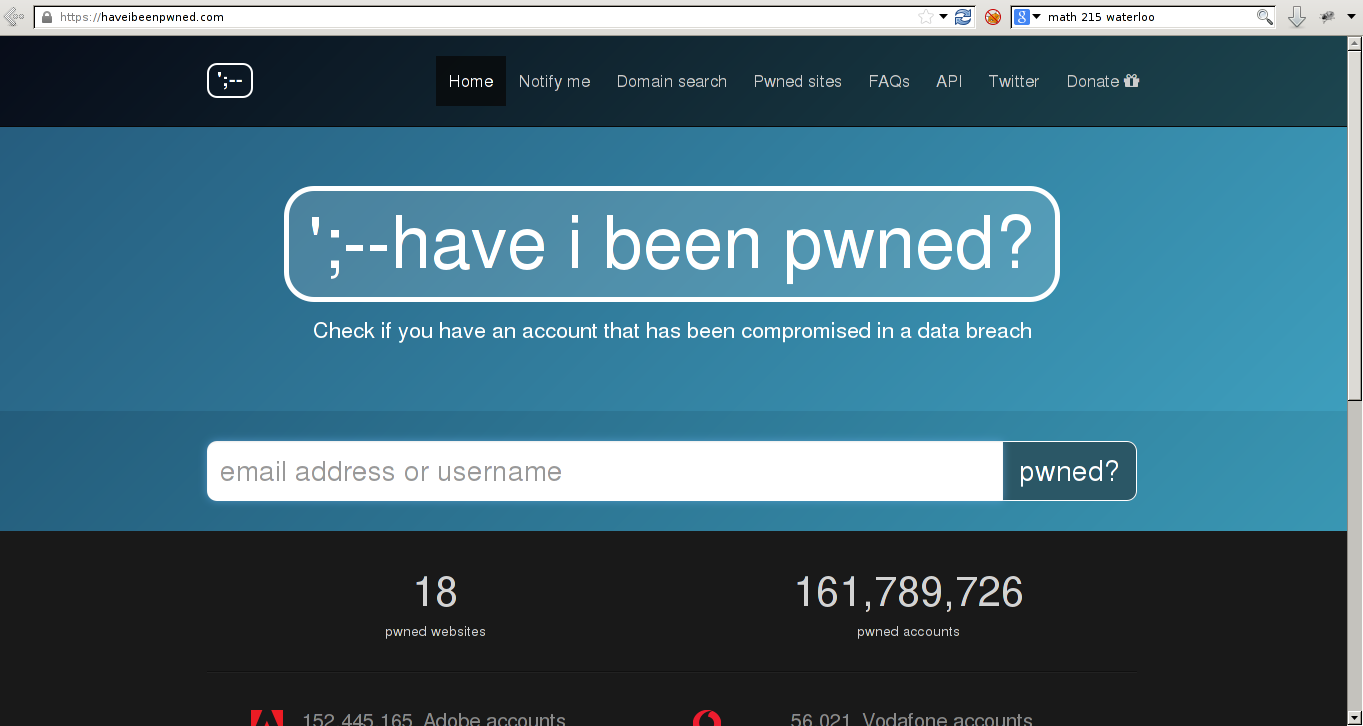
\includegraphics[width=.9\textwidth]{L22/haveibeenpwned.png}
  \end{center}

  Discussion: \\  \hspace*{1em} {\scriptsize \url{http://www.troyhunt.com/2013/12/micro-optimising-web-content-for.html}}
  
\end{frame}
%%%%%%%%%%%%%%%%%%%%%%%%%%%%%%%%%%%%%%%%%%%%%%%%%%%%%%%%%%%%%%%%%%%%%%%%%%%%%%%%

%%%%%%%%%%%%%%%%%%%%%%%%%%%%%%%%%%%%%%%%%%%%%%%%%%%%%%%%%%%%%%%%%%%%%%%%%%%%%%%%
\begin{frame}
  \frametitle{The Issue is Bandwidth}

  \begin{center}
    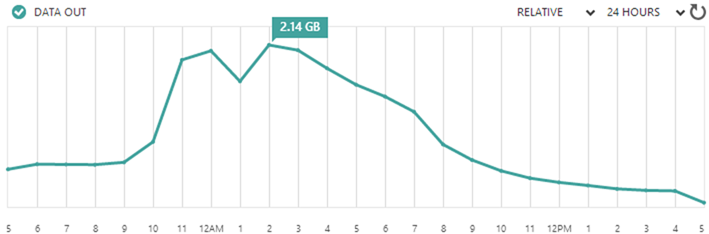
\includegraphics[width=.9\textwidth]{L22/bandwidth-usage.png}
  \end{center}

  \begin{changemargin}{2cm}
  23GB in 24 hours.\\[1em]
  
  This is a problem that you could solve with money. \\ We can do better.
  \end{changemargin}

\end{frame}
%%%%%%%%%%%%%%%%%%%%%%%%%%%%%%%%%%%%%%%%%%%%%%%%%%%%%%%%%%%%%%%%%%%%%%%%%%%%%%%%


%%%%%%%%%%%%%%%%%%%%%%%%%%%%%%%%%%%%%%%%%%%%%%%%%%%%%%%%%%%%%%%%%%%%%%%%%%%%%%%%
\begin{frame}
  \frametitle{Standard Website Tricks}

  \begin{changemargin}{2cm}
    HTML (and JavaScript) + CSS.\\[1em]
    Specifically: Bootstrap, jQuery, Font Awesome.\\
    \hspace*{1em} Bundled and minified.\\
    \hspace*{1em} (2 requests: one for CSS---early, one for JS---late).\\[1em]
    Cache expiration = 1 year; gzip everything.\\[1em]
    5 images: well-optimized SVGs = 12.1kB.\\[1em]
    Disabled all unnecessary response headers.\\[1em]
    Ran through YSlow and Web Page Test (A).
  \end{changemargin}
  
\end{frame}
%%%%%%%%%%%%%%%%%%%%%%%%%%%%%%%%%%%%%%%%%%%%%%%%%%%%%%%%%%%%%%%%%%%%%%%%%%%%%%%%

%%%%%%%%%%%%%%%%%%%%%%%%%%%%%%%%%%%%%%%%%%%%%%%%%%%%%%%%%%%%%%%%%%%%%%%%%%%%%%%%
\begin{frame}
  \frametitle{Conflicting Objectives}

  \begin{changemargin}{1.5cm}
    \begin{itemize}
      \item Speed: load page as fast as possible;
      \item Data volume: minimize outbound data.
    \end{itemize}~\\[1em]

    Example of conflict: \\
    \hspace*{1em} load jQuery from Google's Content Distribution Network, \\
    \hspace*{1em} at the cost of more latency (separate requests).
  \end{changemargin}
  
\end{frame}
%%%%%%%%%%%%%%%%%%%%%%%%%%%%%%%%%%%%%%%%%%%%%%%%%%%%%%%%%%%%%%%%%%%%%%%%%%%%%%%%

%%%%%%%%%%%%%%%%%%%%%%%%%%%%%%%%%%%%%%%%%%%%%%%%%%%%%%%%%%%%%%%%%%%%%%%%%%%%%%%%
\begin{frame}
  \frametitle{About Speed}

  \begin{changemargin}{1.5cm}
    Want site to be ``usable'' as soon as possible.
      \begin{center}
    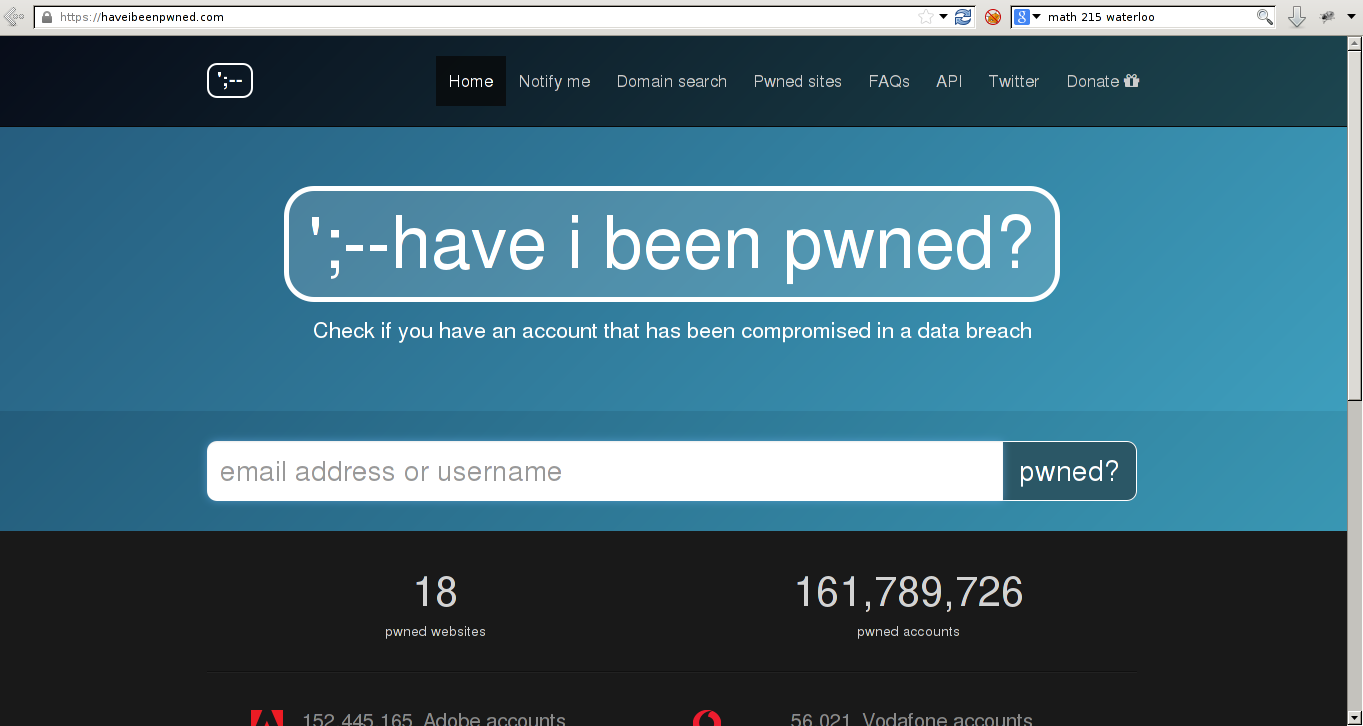
\includegraphics[width=.5\textwidth]{L22/haveibeenpwned.png}
      \end{center}
      \begin{enumerate}
      \item Must load the HTML first (compress it!)
      \item Then you need the CSS.
      \end{enumerate}
      That covers everything except for the logos.\\[1em]
      At this point, the page is ``usable'' (but can't process requests).

  \end{changemargin}
  
\end{frame}
%%%%%%%%%%%%%%%%%%%%%%%%%%%%%%%%%%%%%%%%%%%%%%%%%%%%%%%%%%%%%%%%%%%%%%%%%%%%%%%%

%%%%%%%%%%%%%%%%%%%%%%%%%%%%%%%%%%%%%%%%%%%%%%%%%%%%%%%%%%%%%%%%%%%%%%%%%%%%%%%%
\begin{frame}
  \frametitle{Adding intelligence}

  \begin{changemargin}{2cm}
    To actually start processing, need JavaScript.\\[1em]
    Don't actually need it until user enters an address\\
    \hspace*{1em} (well, also when clicking on a company;)\\
    \hspace*{1em} (but that's not going to happen instantly either.)\\[1em]
    Graceful degradation: \\
    \hspace*{1em} without JS, use form submission and hyperlink.\\[1em]
    Prefetching: \\
    \hspace*{1em} load 17 breaches directly in the HTML.
  \end{changemargin}
  
\end{frame}
%%%%%%%%%%%%%%%%%%%%%%%%%%%%%%%%%%%%%%%%%%%%%%%%%%%%%%%%%%%%%%%%%%%%%%%%%%%%%%%%

%%%%%%%%%%%%%%%%%%%%%%%%%%%%%%%%%%%%%%%%%%%%%%%%%%%%%%%%%%%%%%%%%%%%%%%%%%%%%%%%
\begin{frame}
  \frametitle{Stages of the Load Lifecycle}

  \begin{changemargin}{2cm}
    \begin{enumerate}
    \item Readable
      \item Visually Complete
      \item Functionally Complete
    \end{enumerate}

  \end{changemargin}
  
\end{frame}
%%%%%%%%%%%%%%%%%%%%%%%%%%%%%%%%%%%%%%%%%%%%%%%%%%%%%%%%%%%%%%%%%%%%%%%%%%%%%%%%

%%%%%%%%%%%%%%%%%%%%%%%%%%%%%%%%%%%%%%%%%%%%%%%%%%%%%%%%%%%%%%%%%%%%%%%%%%%%%%%%
\begin{frame}
  \frametitle{Profiling Page Load}
  \begin{changemargin}{2cm}
    Use e.g. Chrome developer tools.
    \begin{itemize}
    \item Size: actual, compressed.
    \item Time: including latency.
    \item Sequencing/staggering of requests: parallelism!
    \end{itemize}~\\[1em]
    31 requests, 174kB transferred.\\
    Page ready after 200ms, complete after 800ms.
    \end{changemargin}
\end{frame}
%%%%%%%%%%%%%%%%%%%%%%%%%%%%%%%%%%%%%%%%%%%%%%%%%%%%%%%%%%%%%%%%%%%%%%%%%%%%%%%%

%%%%%%%%%%%%%%%%%%%%%%%%%%%%%%%%%%%%%%%%%%%%%%%%%%%%%%%%%%%%%%%%%%%%%%%%%%%%%%%%
\begin{frame}
  \frametitle{Content Distribution Networks}

  \begin{changemargin}{2cm}
    Initially: bundle then minify JavaScript---1 request, 88kB.\\[1em]
    Serve jQuery from Google:
    \begin{itemize}
    \item 2 more requests;
    \item increase bytes transferred by 2kB.
    \end{itemize}
    But you've outsourced JS serving;\\
    \hspace*{1em} now only serve 10kB of JS yourself.\\[1em]
    Plus, it's faster: jQuery loaded in parallel, closer to the user, and may be cached.\\[1em]
    Also works for other libraries.
  \end{changemargin}
  
\end{frame}
%%%%%%%%%%%%%%%%%%%%%%%%%%%%%%%%%%%%%%%%%%%%%%%%%%%%%%%%%%%%%%%%%%%%%%%%%%%%%%%%

%%%%%%%%%%%%%%%%%%%%%%%%%%%%%%%%%%%%%%%%%%%%%%%%%%%%%%%%%%%%%%%%%%%%%%%%%%%%%%%%
\begin{frame}
  \frametitle{Other Tweaks}

  \begin{changemargin}{2cm}
    Make SVG files smaller.\\[1em]
    Convert PNG to SVG.\\[1em]
    Serve SVG from CDNs.\\[1em]
    Do work on client-side (email address validation).
  \end{changemargin}
  
\end{frame}
%%%%%%%%%%%%%%%%%%%%%%%%%%%%%%%%%%%%%%%%%%%%%%%%%%%%%%%%%%%%%%%%%%%%%%%%%%%%%%%%


\part{Profiling}
\frame{\partpage}

%%%%%%%%%%%%%%%%%%%%%%%%%%%%%%%%%%%%%%%%%%%%%%%%%%%%%%%%%%%%%%%%%%%%%%%%%%%%%%%%
\begin{frame}
  \frametitle{Introduction to Profiling}

  \begin{changemargin}{2cm}
    So far we've been looking at small problems.\\[1em]
    Must {\bf profile} to see what takes time in a
      large program.\\[1em]
    Two main outputs:
      \begin{itemize}
        \item flat;
        \item call-graph.
      \end{itemize}
~\\[1em]
    \item Two main data gathering methods:
      \begin{itemize}
        \item statistical;
        \item instrumentation.
      \end{itemize}
  \end{changemargin}
\end{frame}
%%%%%%%%%%%%%%%%%%%%%%%%%%%%%%%%%%%%%%%%%%%%%%%%%%%%%%%%%%%%%%%%%%%%%%%%%%%%%%%%

%%%%%%%%%%%%%%%%%%%%%%%%%%%%%%%%%%%%%%%%%%%%%%%%%%%%%%%%%%%%%%%%%%%%%%%%%%%%%%%%
\begin{frame}
  \frametitle{Profiler Outputs}

  \begin{changemargin}{1.5cm}
  {\bf Flat Profiler:}

  \begin{itemize}
    \item Only computes the average time in a particular function.
    \item Does not include other (useful) information, like callees.
  \end{itemize}

~\\[1em]

  {\bf Call-graph Profiler:}

  \begin{itemize}
    \item Computes call times.
    \item Reports frequency of function calls.
    \item Gives a call graph: who called what function?
  \end{itemize}
  \end{changemargin}
\end{frame}
%%%%%%%%%%%%%%%%%%%%%%%%%%%%%%%%%%%%%%%%%%%%%%%%%%%%%%%%%%%%%%%%%%%%%%%%%%%%%%%%

%%%%%%%%%%%%%%%%%%%%%%%%%%%%%%%%%%%%%%%%%%%%%%%%%%%%%%%%%%%%%%%%%%%%%%%%%%%%%%%%
\begin{frame}
  \frametitle{Data Gathering Methods}

  \begin{changemargin}{2cm}
  {\bf Statistical:}

  Mostly, take samples of the system state, that is:
  \begin{itemize}
    \item every 2ns, check the system state.
    \item will cause some slowdown, but not much.
  \end{itemize}
~\\[1em]

  {\bf Instrumentation:}\\
  Add additional instructions at specified program points:
  \begin{itemize}
    \item can do this at compile time or run time (expensive);
    \item can instrument either manually or automatically;
    \item like conditional breakpoints.
  \end{itemize}
  \end{changemargin}
\end{frame}
%%%%%%%%%%%%%%%%%%%%%%%%%%%%%%%%%%%%%%%%%%%%%%%%%%%%%%%%%%%%%%%%%%%%%%%%%%%%%%%%

%%%%%%%%%%%%%%%%%%%%%%%%%%%%%%%%%%%%%%%%%%%%%%%%%%%%%%%%%%%%%%%%%%%%%%%%%%%%%%%%
\begin{frame}
  \frametitle{Guide to Profiling}

  \begin{changemargin}{1cm}
  When writing large software projects:
  \begin{itemize}
    \item First, write clear and concise code. \\
      Don't do any premature optimizations---focus on correctness.
    \item Profile to get a baseline of your performance:
      \begin{itemize}
        \item allows you to easily track any performance changes;
        \item allows you to re-design your program before it's too late.
      \end{itemize}
  \end{itemize}
  Focus your optimization efforts on the code that matters.
  \end{changemargin}
\end{frame}
%%%%%%%%%%%%%%%%%%%%%%%%%%%%%%%%%%%%%%%%%%%%%%%%%%%%%%%%%%%%%%%%%%%%%%%%%%%%%%%%

%%%%%%%%%%%%%%%%%%%%%%%%%%%%%%%%%%%%%%%%%%%%%%%%%%%%%%%%%%%%%%%%%%%%%%%%%%%%%%%%
\begin{frame}
  \frametitle{Things to Look For}

  \begin{changemargin}{1.5cm}
    Good signs:

    \begin{itemize}
      \item Time is spent in the right part of the system.
      \item Most time should not be spent handling errors; in
      non-critical code; or in exceptional cases.
      \item Time is not unnecessarily spent in the operating system.
    \end{itemize}
  \end{changemargin}
\end{frame}
%%%%%%%%%%%%%%%%%%%%%%%%%%%%%%%%%%%%%%%%%%%%%%%%%%%%%%%%%%%%%%%%%%%%%%%%%%%%%%%%

%%%%%%%%%%%%%%%%%%%%%%%%%%%%%%%%%%%%%%%%%%%%%%%%%%%%%%%%%%%%%%%%%%%%%%%%%%%%%%%%
\begin{frame}
  \frametitle{{\tt gprof} introduction}

  \begin{changemargin}{2cm}
    Statistical profiler, plus some instrumentation for calls.\\[1em]
    Runs completely in user-space.\\[1em]
    Only requires a compiler.
  \end{changemargin}
\end{frame}
%%%%%%%%%%%%%%%%%%%%%%%%%%%%%%%%%%%%%%%%%%%%%%%%%%%%%%%%%%%%%%%%%%%%%%%%%%%%%%%%

%%%%%%%%%%%%%%%%%%%%%%%%%%%%%%%%%%%%%%%%%%%%%%%%%%%%%%%%%%%%%%%%%%%%%%%%%%%%%%%%
\begin{frame}
  \frametitle{{\tt gprof} usage}

  \begin{changemargin}{2cm}
    Use the {\tt -pg} flag with {\tt gcc} when compiling and linking.\\[1em]
    Run your program as you normally would.
      \begin{itemize}
        \item Your program will now create a {\tt gmon.out} file.
      \end{itemize}
~\\
    \item Use gprof to interpret the results: {\tt gprof <executable>}.
  \end{changemargin}
\end{frame}
%%%%%%%%%%%%%%%%%%%%%%%%%%%%%%%%%%%%%%%%%%%%%%%%%%%%%%%%%%%%%%%%%%%%%%%%%%%%%%%%

%%%%%%%%%%%%%%%%%%%%%%%%%%%%%%%%%%%%%%%%%%%%%%%%%%%%%%%%%%%%%%%%%%%%%%%%%%%%%%%%
\begin{frame}[fragile]
  \frametitle{{\tt gprof} example}

  \begin{changemargin}{1.5cm}
    A program with 100 million calls to two math functions.

  \begin{lstlisting}
int main() {
    int i,x1=10,y1=3,r1=0;
    float x2=10,y2=3,r2=0;

    for(i=0;i<100000000;i++) {
        r1 += int_math(x1,y1);
        r2 += float_math(y2,y2);
    }
}
  \end{lstlisting}

  \begin{itemize}
    \item Looking at the code, we have no idea what takes longer.
    \item Probably would guess floating point math taking longer.
    \item (Overall, silly example.)
  \end{itemize}
  \end{changemargin}
\end{frame}
%%%%%%%%%%%%%%%%%%%%%%%%%%%%%%%%%%%%%%%%%%%%%%%%%%%%%%%%%%%%%%%%%%%%%%%%%%%%%%%%

%%%%%%%%%%%%%%%%%%%%%%%%%%%%%%%%%%%%%%%%%%%%%%%%%%%%%%%%%%%%%%%%%%%%%%%%%%%%%%%%
\begin{frame}[fragile]
  \frametitle{Example (Integer Math)}

  \begin{changemargin}{1.5cm}
  \begin{lstlisting}
int int_math(int x, int y){
    int r1;
    r1=int_power(x,y);
    r1=int_math_helper(x,y);
    return r1;
}

int int_math_helper(int x, int y){
    int r1;
    r1=x/y*int_power(y,x)/int_power(x,y);
    return r1;
}

int int_power(int x, int y){
    int i, r;
    r=x;
    for(i=1;i<y;i++){
        r=r*x;
    }
    return r;
}
  \end{lstlisting}
  \end{changemargin}
\end{frame}
%%%%%%%%%%%%%%%%%%%%%%%%%%%%%%%%%%%%%%%%%%%%%%%%%%%%%%%%%%%%%%%%%%%%%%%%%%%%%%%%


%%%%%%%%%%%%%%%%%%%%%%%%%%%%%%%%%%%%%%%%%%%%%%%%%%%%%%%%%%%%%%%%%%%%%%%%%%%%%%%%
\begin{frame}[fragile]
  \frametitle{Example (Float Math)}

  \begin{changemargin}{2cm}
  \begin{lstlisting}
float float_math(float x, float y) {
    float r1;
    r1=float_power(x,y);
    r1=float_math_helper(x,y);
    return r1;
}

float float_math_helper(float x, float y) {
    float r1;
    r1=x/y*float_power(y,x)/float_power(x,y);
    return r1;
}

float float_power(float x, float y){
    float i, r;
    r=x;
    for(i=1;i<y;i++) {
        r=r*x;
    }
    return r;
}
  \end{lstlisting}
  \end{changemargin}
\end{frame}
%%%%%%%%%%%%%%%%%%%%%%%%%%%%%%%%%%%%%%%%%%%%%%%%%%%%%%%%%%%%%%%%%%%%%%%%%%%%%%%%

%%%%%%%%%%%%%%%%%%%%%%%%%%%%%%%%%%%%%%%%%%%%%%%%%%%%%%%%%%%%%%%%%%%%%%%%%%%%%%%%
\begin{frame}[fragile]
  \frametitle{Flat Profile}

\begin{changemargin}{1cm}
    When we run the program and look at the profile, we see:

{
  \begin{lstlisting}[basicstyle=\tiny]
Flat profile:

Each sample counts as 0.01 seconds.
  %   cumulative   self              self     total           
 time   seconds   seconds    calls  ns/call  ns/call  name    
 32.58      4.69     4.69 300000000    15.64    15.64  int_power
 30.55      9.09     4.40 300000000    14.66    14.66  float_power
 16.95     11.53     2.44 100000000    24.41    55.68  int_math_helper
 11.43     13.18     1.65 100000000    16.46    45.78  float_math_helper
  4.05     13.76     0.58 100000000     5.84    77.16  int_math
  3.01     14.19     0.43 100000000     4.33    64.78  float_math
  2.10     14.50     0.30                             main
  \end{lstlisting}
}

  \begin{itemize}
    \item One function per line.
    \item {\bf \% time:} the percent of the total execution time in this function.
    \item {\bf self:} seconds in this function.
    \item {\bf cumulative:} sum of this function's time + any above it in table.
  \end{itemize}
\end{changemargin}
\end{frame}
%%%%%%%%%%%%%%%%%%%%%%%%%%%%%%%%%%%%%%%%%%%%%%%%%%%%%%%%%%%%%%%%%%%%%%%%%%%%%%%%

%%%%%%%%%%%%%%%%%%%%%%%%%%%%%%%%%%%%%%%%%%%%%%%%%%%%%%%%%%%%%%%%%%%%%%%%%%%%%%%%
\begin{frame}[fragile]
  \frametitle{Flat Profile}

\begin{changemargin}{1cm}
  \begin{lstlisting}[basicstyle=\tiny]
Flat profile:

Each sample counts as 0.01 seconds.
  %   cumulative   self              self     total           
 time   seconds   seconds    calls  ns/call  ns/call  name    
 32.58      4.69     4.69 300000000    15.64    15.64  int_power
 30.55      9.09     4.40 300000000    14.66    14.66  float_power
 16.95     11.53     2.44 100000000    24.41    55.68  int_math_helper
 11.43     13.18     1.65 100000000    16.46    45.78  float_math_helper
  4.05     13.76     0.58 100000000     5.84    77.16  int_math
  3.01     14.19     0.43 100000000     4.33    64.78  float_math
  2.10     14.50     0.30                             main
  \end{lstlisting}


  \begin{itemize}
    \item {\bf calls:} number of times this function was called
    \item {\bf self ns/call:} just self nanoseconds / calls
    \item {\bf total ns/call:} average time for function execution, including
      any other calls the function makes
  \end{itemize}
\end{changemargin}
\end{frame}
%%%%%%%%%%%%%%%%%%%%%%%%%%%%%%%%%%%%%%%%%%%%%%%%%%%%%%%%%%%%%%%%%%%%%%%%%%%%%%%%

%%%%%%%%%%%%%%%%%%%%%%%%%%%%%%%%%%%%%%%%%%%%%%%%%%%%%%%%%%%%%%%%%%%%%%%%%%%%%%%%
\begin{frame}[fragile]
  \frametitle{Call Graph Example (1)}

  \begin{changemargin}{1cm}
    After the flat profile gives you a feel for which functions are costly, you
      can get a better story from the call graph.
  \vfill
  \begin{lstlisting}[basicstyle=\tiny]
index % time    self  children    called     name
                                                 <spontaneous>
[1]    100.0    0.30   14.19                 main [1]
                0.58    7.13 100000000/100000000     int_math [2]
                0.43    6.04 100000000/100000000     float_math [3]
-----------------------------------------------
                0.58    7.13 100000000/100000000     main [1]
[2]     53.2    0.58    7.13 100000000         int_math [2]
                2.44    3.13 100000000/100000000     int_math_helper [4]
                1.56    0.00 100000000/300000000     int_power [5]
-----------------------------------------------
                0.43    6.04 100000000/100000000     main [1]
[3]     44.7    0.43    6.04 100000000         float_math [3]
                1.65    2.93 100000000/100000000     float_math_helper [6]
                1.47    0.00 100000000/300000000     float_power [7]
  \end{lstlisting}
  \end{changemargin}
\end{frame}
%%%%%%%%%%%%%%%%%%%%%%%%%%%%%%%%%%%%%%%%%%%%%%%%%%%%%%%%%%%%%%%%%%%%%%%%%%%%%%%%

%%%%%%%%%%%%%%%%%%%%%%%%%%%%%%%%%%%%%%%%%%%%%%%%%%%%%%%%%%%%%%%%%%%%%%%%%%%%%%%%
\begin{frame}[fragile]
  \frametitle{Reading the Call Graph}

  \begin{changemargin}{1.5cm}
    The line with the index is the current function being looked at\\
      \qquad \qquad {\bf (primary line)}.\\
\begin{itemize}
    \item Lines above are functions which called this function.
    \item Lines below are functions which were called by this function
      (children).
  \end{itemize}
~\\
  {\bf Primary Line}

  \begin{itemize}  
    \item {\bf time:} total percentage of time spent in this function and its
      children
    \item {\bf self:} same as in flat profile
    \item {\bf children:} time spent in all calls made by the function
      \begin{itemize}
        \item should be equal to self + children of all functions below
      \end{itemize}
  \end{itemize}
  \end{changemargin}
\end{frame}
%%%%%%%%%%%%%%%%%%%%%%%%%%%%%%%%%%%%%%%%%%%%%%%%%%%%%%%%%%%%%%%%%%%%%%%%%%%%%%%%

%%%%%%%%%%%%%%%%%%%%%%%%%%%%%%%%%%%%%%%%%%%%%%%%%%%%%%%%%%%%%%%%%%%%%%%%%%%%%%%%
\begin{frame}[fragile]
  \frametitle{Reading Callers from Call Graph}

  \begin{changemargin}{2cm}
  {\bf Callers (functions above the primary line)}
  \begin{itemize}  
    \item {\bf self:} time spent in primary function, when called from current
      function.
    \item {\bf children:} time spent in primary function's children, when
      called from current function.
    \item {\bf called:} number of times primary function was called from current
      function / number of nonrecursive calls to primary function.
  \end{itemize}
  \end{changemargin}
\end{frame}
%%%%%%%%%%%%%%%%%%%%%%%%%%%%%%%%%%%%%%%%%%%%%%%%%%%%%%%%%%%%%%%%%%%%%%%%%%%%%%%%

%%%%%%%%%%%%%%%%%%%%%%%%%%%%%%%%%%%%%%%%%%%%%%%%%%%%%%%%%%%%%%%%%%%%%%%%%%%%%%%%
\begin{frame}[fragile]
  \frametitle{Reading Callees from Call Graph}

  \begin{changemargin}{1cm}
  {\bf Callees (functions below the primary line)}
  \begin{itemize}  
    \item {\bf self:} time spent in current function when called from primary.
    \item {\bf children:} time spent in current function's children calls when
      called from primary.
      \begin{itemize}
        \item self + children is an estimate of time spent in current function
          when called from primary function.
      \end{itemize}
    \item {\bf called:} number of times current function was called from primary
      function / number of nonrecursive calls to current function.
  \end{itemize}
  \end{changemargin}
\end{frame}
%%%%%%%%%%%%%%%%%%%%%%%%%%%%%%%%%%%%%%%%%%%%%%%%%%%%%%%%%%%%%%%%%%%%%%%%%%%%%%%%

%%%%%%%%%%%%%%%%%%%%%%%%%%%%%%%%%%%%%%%%%%%%%%%%%%%%%%%%%%%%%%%%%%%%%%%%%%%%%%%%
\begin{frame}[fragile]
  \frametitle{Call Graph Example (2)}

  \begin{changemargin}{1cm}
  \begin{lstlisting}[basicstyle=\tiny]
index % time    self  children    called     name

                2.44    3.13 100000000/100000000     int_math [2]
[4]     38.4    2.44    3.13 100000000         int_math_helper [4]
                3.13    0.00 200000000/300000000     int_power [5]
-----------------------------------------------
                1.56    0.00 100000000/300000000     int_math [2]
                3.13    0.00 200000000/300000000     int_math_helper [4]
[5]     32.4    4.69    0.00 300000000         int_power [5]
-----------------------------------------------
                1.65    2.93 100000000/100000000     float_math [3]
[6]     31.6    1.65    2.93 100000000         float_math_helper [6]
                2.93    0.00 200000000/300000000     float_power [7]
-----------------------------------------------
                1.47    0.00 100000000/300000000     float_math [3]
                2.93    0.00 200000000/300000000     float_math_helper [6]
[7]     30.3    4.40    0.00 300000000         float_power [7]
  \end{lstlisting}

  
 We can now see where most of the time comes from, and pinpoint any
      locations that make unexpected calls, etc.\\[1em]
 This example isn't too exciting; we could simplify the math.
  \end{changemargin}
\end{frame}
%%%%%%%%%%%%%%%%%%%%%%%%%%%%%%%%%%%%%%%%%%%%%%%%%%%%%%%%%%%%%%%%%%%%%%%%%%%%%%%%

%%%%%%%%%%%%%%%%%%%%%%%%%%%%%%%%%%%%%%%%%%%%%%%%%%%%%%%%%%%%%%%%%%%%%%%%%%%%%%%%
\begin{frame}
  \frametitle{Summary (Profiling)}

  \begin{changemargin}{1cm}
  \begin{itemize}
    \item Saw how to use {\tt gprof} \\ \qquad (one option for Assignment 3).
    \item Profile early and often.
    \item Make sure your profiling shows what you expect. 
  \end{itemize}
  \end{changemargin}
\end{frame}
%%%%%%%%%%%%%%%%%%%%%%%%%%%%%%%%%%%%%%%%%%%%%%%%%%%%%%%%%%%%%%%%%%%%%%%%%%%%%%%%

\end{document}
